\chapter{Gráfanalitikai eredmények: asszortativitás és betweenness centralitás}

A PremadeGraph két fő gráfanalitikai modulja az asszortativitás és a Brandes-féle betweenness centralitás. Mindkettő a Rust futtatókörnyezetben van implementálva, a frontend dedikált analitikai oldalakon jeleníti meg az eredményeket. Az asszortativitás azt vizsgálja, hogy az összekapcsolt játékosok hasonló teljesítményprofilhoz tartoznak-e; a betweenness centralitás azt méri, hogy egyes csomópontok hány legrövidebb úton helyezkednek el, tehát topológiai bróker-szerepet töltenek-e be.

\section{Asszortativitás}

\subsection{A számítási definíció}

A jelenlegi implementáció numerikus asszortativitást számol Pearson-korreláció formájában. Ha az él egyik végpontján mért értékeket $x_i$, a másik végpontén mért értékeket pedig $y_i$ jelöli, akkor az együttható:

\begin{equation}
r = \frac{\sum_i (x_i-\bar{x})(y_i-\bar{y})}{\sqrt{\sum_i (x_i-\bar{x})^2}\sqrt{\sum_i (y_i-\bar{y})^2}}
\end{equation}

Az irányítatlan éleket az implementáció mindkét endpoint-orientációval figyelembe veszi a Pearson-akkumulációban, mert az élnek nincs természetes iránya, és a két végpont tulajdonságpárja szimmetrikusan járul hozzá a korrelációhoz. A modul emellett külön számolja az alacsony támogatás, a hiányzó score és a túl rövid játékostörténet miatt kihagyott éleket, így az asszortativitási eredmény nem feketedoboz-korreláció, hanem dokumentált mintaképzési folyamat eredménye.

\begin{figure}[h]
\centering
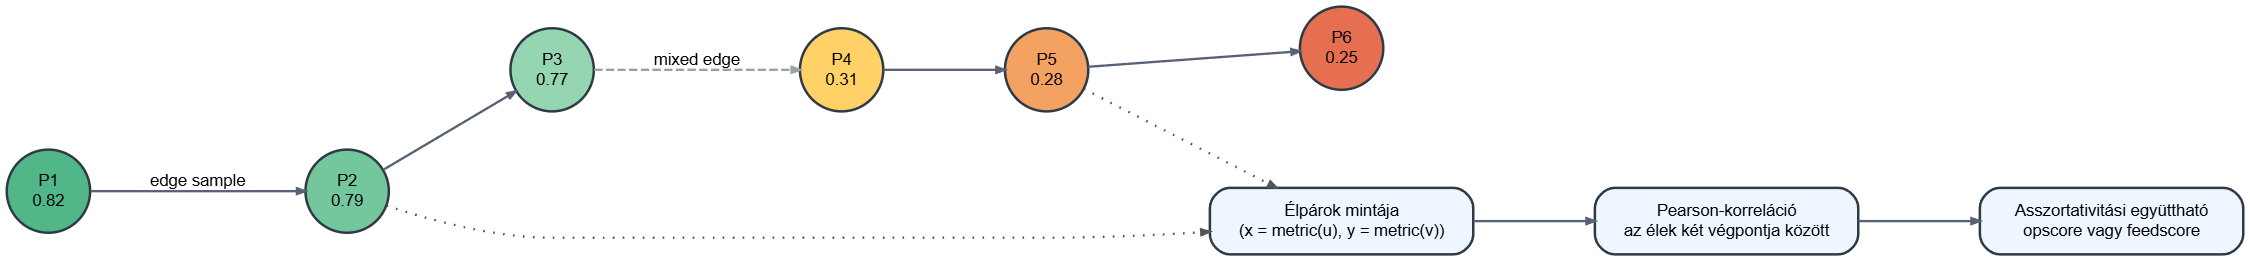
\includegraphics[width=0.92\textwidth]{assets/diagrams/thesis_assortativity_graphviz.png}
\caption{Az asszortativitás él-végponti értelmezése: az összekapcsolt játékospárok metrikaértékei Pearson-korrelációként kerülnek összesítésre.}
\label{fig:assortativity-graphviz-overview}
\end{figure}

\begin{figure}[H]
\centering

\includegraphics[width=0.98\textwidth,height=0.30\textheight,keepaspectratio]{assortavity-controls.png}
\caption{Az asszortativitási kísérlet frontend kontrolljai. A képen a minimum éltámogatás, a minimum játékos-meccsszám és az erős kapcsolat küszöbe látható; a bemutatott futtatásokban ezek rendre 1, 1 és 3 értékkel szerepelnek.}
\end{figure}

\begin{figure}[H]
\centering

\includegraphics[width=0.98\textwidth,height=0.48\textheight,keepaspectratio]{assortavity-documented-desicions.png}
\caption{A frontend által megjelenített dokumentált módszertani döntések. A képernyő rögzíti, hogy Pearson endpoint-korrelációt használunk, a \textit{social-path} és \textit{battle-path} módokat külön kezeljük, a metrikák az \textit{opscore} és \textit{feedscore}, és csak azok a végpontok maradnak a mintában, amelyekhez érvényes metrika és elegendő meccstörténet tartozik.}
\end{figure}

\subsection{Él-végponti minta kiválasztása}

A Pearson-korreláció az élek között számítódik. Az implementáció az összes élt végigfuttatja az aktuális gráfmódnak megfelelő szűrőn, majd minden élhez lekérdezi az egyik és a másik végpont \textit{opscore} vagy \textit{feedscore} értékét. Ha bármelyik score hiányzik, vagy ha valamelyik játékos \textit{match\_count} értéke a minimum alá esik, az él kiesik. A maradék élek score-párjai képezik az akkumulált vektorokat. Ez a szűrés olyan mintahalmazt eredményez, amely az erős kapcsolatok körül tömörödik: az asszortativitás nem „mindent figyelembe vevő" globális mérőszám, hanem a releváns kapcsolathálózat szerkezeti tulajdonsága.

\subsection{Gráfmód-specifikus él-súlyozás}

A gráfmód alapján az él-súlyozás a következőképpen alakul:

\begin{equation}
w(u,v) = \begin{cases}
\textit{ally\_weight} & \text{ha } \textit{social-path} \\
\textit{total\_matches} & \text{ha } \textit{battle-path}
\end{cases}
\end{equation}

A \textit{social-path} módban csak a szövetségesi kapcsolatok sugallják az él meglétét; a \textit{battle-path} módban az összes ismétlődés (szövetséges és ellenséges) beszámít. Ez a különbség eltérő társas szerkezeti hipotéziseket tesztel: a social-path azt kérdezi, hogy a szövetségesi hálózatban csoportosulnak-e a hasonló teljesítmények, a battle-path pedig azt, hogy az összes ismétlődő kapcsolaton korrálnak-e.

\subsection{Bontások és hiányzó adat kezelése}

Az implementáció globális korreláción túl klaszteren belüli és klaszterek közötti, valamint erős és gyenge kapcsolatok szerinti bontást is képez. Ha a within-cluster érték magasabb, az a klasztertagok hasonló teljesítményprofilját jelzi; ha a between-cluster is magas, az asszortativitás klaszter-független tulajdonság. Hiányzó score-ok esetén az alapértelmezett \textit{skip} politika az óvatos választás: nem extrapolálunk hiányzó adatokra, így az eredmény az „amit ténylegesen tudunk" alapon számítódik.

\section{Asszortativitási eredmények}

\subsection{Flexset}

\begin{table}[H]
\centering
\caption{Asszortativitás - \textit{flexset}}
\begin{tabular}{llrr}
\toprule
\textbf{Gráfmód} & \textbf{Metrika} & \textbf{Korreláció} & \textbf{Mintaszám} \\
\midrule
\textit{social-path} & \textit{opscore} & 0.2346 & 61\,938 \\
\textit{social-path} & \textit{feedscore} & 0.1816 & 61\,938 \\
\textit{battle-path} & \textit{opscore} & 0.1461 & 179\,492 \\
\textit{battle-path} & \textit{feedscore} & $-0.0108$ & 179\,492 \\
\bottomrule
\end{tabular}
\end{table}

\begin{figure}[H]
\centering

\includegraphics[width=0.98\textwidth,height=0.74\textheight,keepaspectratio]{f-assortavity-social-path-opfeedscore.png}
\caption{\textit{flexset} social-path asszortativitás \textit{opscore} és \textit{feedscore} szerint. A képen 15\,421 jogosult csomópont és 61\,938 elemzett él szerepel; a globális együttható \textit{opscore} esetén 0.235, \textit{feedscore} esetén 0.182. A bontások azt mutatják, hogy a kereszt-klaszter élek erősebb pozitív jelet adnak, mint a klaszteren belüli élek, miközben a gyenge kapcsolatok nagy mintaszámmal hordozzák a pozitív mintázatot.}
\end{figure}

\begin{figure}[H]
\centering

\includegraphics[width=0.98\textwidth,height=0.52\textheight,keepaspectratio]{f-assortavity-socialpath-readout.png}
\caption{\textit{flexset} social-path technikai readout. A sávos összehasonlítás a globális, within-cluster, cross-cluster, strong-tie és weak-tie bontásokat teszi egymás mellé; látható, hogy az \textit{opscore} minden bontásban pozitív, a \textit{feedscore} pedig social-path módban szintén pozitív marad.}
\end{figure}

\begin{figure}[H]
\centering

\includegraphics[width=0.98\textwidth,height=0.74\textheight,keepaspectratio]{f-assortavity-battle-path-opfeedscore.png}
\caption{\textit{flexset} battle-path asszortativitás \textit{opscore} és \textit{feedscore} szerint. A képen ugyanaz a 15\,421 jogosult csomópont, de már 179\,492 elemzett él látható; a \textit{battle-path} mód több kapcsolatot vesz be, ezért az \textit{opscore} jel 0.146-ra gyengül, a \textit{feedscore} pedig gyakorlatilag nullára esik ($-0.011$).}
\end{figure}

\begin{figure}[H]
\centering

\includegraphics[width=0.98\textwidth,height=0.36\textheight,keepaspectratio]{f-assortavity-battlepath-readout.png}
\caption{\textit{flexset} battle-path technikai readout. A képernyőn az látszik, hogy a battle-path \textit{opscore} pozitív, de mérsékeltebb hasonlósági jelet ad, míg a \textit{feedscore} globálisan és a gyenge kapcsolatokon közel nulla vagy enyhén negatív.}
\end{figure}

\begin{figure}[H]
\centering

\includegraphics[width=0.98\textwidth,height=0.38\textheight,keepaspectratio]{f-assortavity-layman-takeaways.png}
\caption{\textit{flexset} közérthető frontend-összegzés. A képernyő azt emeli ki, hogy a kapcsolt játékosok \textit{opscore} szerint mindkét gráfmódban hasonlóbbak, a \textit{feedscore} viszont erősen gráfmód-függő; a következtetés leíró hálózati szerkezetről szól, nem oksági vagy pszichológiai állításról.}
\end{figure}

A \textit{flexset} legfontosabb tanulsága: a szövetségesi kapcsolatokra épülő social-path gráfban jelenik meg a legerősebb teljesítményhasonlósági jel. Ez illeszkedik ahhoz az értelmezéshez, hogy a Flex Queue nem pusztán véletlen matchmaking-minta. A cross-cluster \textit{opscore} érték magasabb, mint a within-cluster érték, tehát az asszortativitás nem egyszerűen a klaszterezés mellékterméke: a határkapcsolatokban is mérhető.

\subsection{SoloQ}

\begin{table}[H]
\centering
\caption{Asszortativitás - \textit{soloq}}
\begin{tabular}{llrr}
\toprule
\textbf{Gráfmód} & \textbf{Metrika} & \textbf{Korreláció} & \textbf{Mintaszám} \\
\midrule
\textit{social-path} & \textit{opscore} & 0.1750 & 37\,976 \\
\textit{social-path} & \textit{feedscore} & 0.1012 & 37\,976 \\
\textit{battle-path} & \textit{opscore} & 0.1625 & 84\,393 \\
\textit{battle-path} & \textit{feedscore} & $-0.0366$ & 84\,393 \\
\bottomrule
\end{tabular}
\end{table}

\begin{figure}[H]
\centering

\includegraphics[width=0.98\textwidth,height=0.74\textheight,keepaspectratio]{sq-assortavity-social-path-opfeedscore.png}
\caption{\textit{soloq} social-path asszortativitás \textit{opscore} és \textit{feedscore} szerint. A képen 6\,768 jogosult csomópont és 37\,976 elemzett él szerepel; a globális együttható \textit{opscore} esetén 0.175, \textit{feedscore} esetén 0.101. A pozitív értékek megmaradnak, de gyengébbek, mint a \textit{flexset} social-path eredményei.}
\end{figure}

\begin{figure}[H]
\centering

\includegraphics[width=0.98\textwidth,height=0.36\textheight,keepaspectratio]{sq-assortavity-socialpath-readout.png}
\caption{\textit{soloq} social-path technikai readout. A sávos nézet azt mutatja, hogy a cross-cluster bontás adja a legerősebb pozitív jelet, míg a within-cluster értékek közel semlegesek; a strong-tie minta különösen kicsi, ezért ebben a datasetben óvatosan értelmezendő.}
\end{figure}

\begin{figure}[H]
\centering

\includegraphics[width=0.98\textwidth,height=0.74\textheight,keepaspectratio]{sq-assortavity-battle-path-opfeedscore.png}
\caption{\textit{soloq} battle-path asszortativitás \textit{opscore} és \textit{feedscore} szerint. A képen 84\,393 elemzett él látható; az \textit{opscore} globálisan 0.163 marad, a \textit{feedscore} viszont $-0.037$ értékre fordul.}
\end{figure}

\begin{figure}[H]
\centering

\includegraphics[width=0.98\textwidth,height=0.36\textheight,keepaspectratio]{sq-assortavity-battlepath-readout.png}
\caption{\textit{soloq} battle-path technikai readout. A képernyőn az \textit{opscore} pozitív, de mérsékelt értékei látszanak, míg a \textit{feedscore} globálisan, within-cluster és cross-cluster bontásban is negatív közeli értékeket vesz fel.}
\end{figure}

\begin{figure}[H]
\centering

\includegraphics[width=0.98\textwidth,height=0.58\textheight,keepaspectratio]{sq-assortavity-layman-takeaways.png}
\caption{\textit{soloq} közérthető frontend-összegzés. A képernyő azt foglalja össze, hogy az \textit{opscore} hasonlóság mindkét gráfmódban megmarad, de a \textit{feedscore} jelentősen változik; a módszertani panel külön jelzi, hogy a minimum support, a minimum meccsszám és az erős kapcsolat küszöbe befolyásolja, mennyire konzervatív a futtatás.}
\end{figure}

A \textit{soloq} kontrollszerepe itt látszik: a pozitív \textit{opscore} asszortativitás nem tűnik el, tehát a teljesítményhasonlósági jel nem kizárólag Flex Queue sajátosság. Ugyanakkor a social-path érték alacsonyabb, a strong-tie minták kicsik, és a \textit{feedscore} battle-path módban negatív közeli eredményt ad. Ez azt támasztja alá, hogy a SoloQ inkább egyéni teljesítmény- és matchmaking-rekurrencia kontrollként értelmezhető, nem stabil premade-kapcsolati hálóként.

\subsection{Értelmezés}

Mindkét datasetben pozitív asszortativitás jelenik meg az \textit{opscore} mentén a \textit{social-path} módban, ami azt jelzi, hogy a szövetségesi kapcsolatokra épülő gráfban az összekapcsolt játékosok teljesítményprofilja nem véletlenszerűen keveredik. A \textit{feedscore} viselkedése jóval érzékenyebb a gráfmódra: social-path módban mindkét dataseten mérsékelt pozitív jel látható, de battle-path módban közel nullára esik (flexset: $-0.0108$, soloq: $-0.0366$). Az ellenfélkapcsolatok bevonásával a halálokon alapuló hibamutató elveszíti a társas-kapcsolati hasonlósági szerkezetet.

A flexset social-path \textit{opscore} asszortativitás (0.2346) magasabb, mint a soloq-é (0.1750), ami összhangban van azzal, hogy a Flex Queue erősebb visszatérő csapattársi szignált hoz létre. A battle-path mód mindkét datasetben lényegesen több élt vizsgál, de ez nem erősíti a korrelációt: a flexset esetén az élminta 61\,938-ról 179\,492-re nő, mégis csökken az \textit{opscore} asszortativitás és eltűnik a \textit{feedscore} jel. Több él nem automatikusan jobb bizonyíték, ha az élhalmaz szemantikája kevertebb.

Az \textit{opscore} minden vizsgált módban pozitív marad, a \textit{feedscore} nem; ez a kompozit mutató erőssége az egyszerűbb halálközpontú képlettel szemben. Nem azt állítjuk, hogy az \textit{opscore} objektív igazság, de empirikusan megmutatja, hogy a gráf és a score-réteg között érdemi kapcsolat van, és ez gráfmódváltáskor sem tűnik el. A gráfmód-érzékenység módszertani eredmény önmagában is: ha mindkét metrika minden módban azonos értéket adna, a gráfdefiníció nem hordozna önálló tartalmat. Az \textit{opscore} csökkenése battle-path módban és a \textit{feedscore} nullára esése azt mutatja, hogy a kapcsolatok szemantikája meghatározza a teljesítményhasonlóság mérhetőségét, és a két gráfmód megkülönböztetése empirikusan indokolt módszertani döntés.

A randomizációs szignifikanciateszt infrastruktúrája megvan a rendszerben, de a jelen dolgozatban a fő eredmények a közvetlenül ellenőrzött leíró és bontott futtatásokon alapulnak.

\section{Betweenness centralitás}

A bridge-orbit vizualizáció a Graph V2 pipeline-ból heurisztikus pontszámokkal (\textit{orbitScore}, \textit{orbitRadius}) azonosít egyes csomópontokat és klasztereket hidaknak. Ezek a mezők azonban vizuális heurisztikák: a kereszt-klaszter szövetségesi támasz, az összekötött klasztercsoport-szám és a tagszám kombinációján alapulnak, de nem ellenőrzik, hogy a jelölt csomópontok valóban a legtöbb legrövidebb útvonal metszéspontján helyezkednek-e el. A Brandes-féle betweenness centralitás éppen ezt az ellenőrzést teszi lehetővé: teljes gráfbejáráson alapul, nem becslésen.

\begin{figure}[h]
\centering
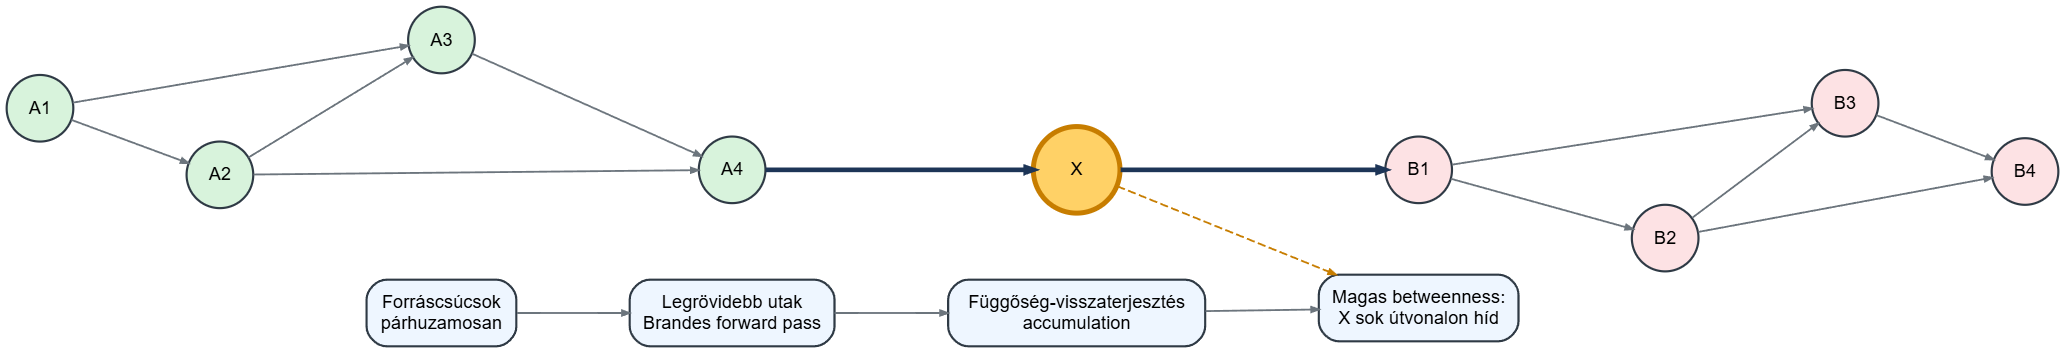
\includegraphics[width=0.92\textwidth]{assets/diagrams/thesis_brandes_bridge_graphviz.png}
\caption{A betweenness centralitás intuitív értelmezése: a hídcsomópont sok klaszterközi legrövidebb útvonalon jelenik meg, ezért magas Brandes-pontszámot kap.}
\label{fig:brandes-bridge-graphviz}
\end{figure}

\subsection{A Brandes-algoritmus}

A Brandes-algoritmus \cite{brandes2001} a hagyományos $O(n^3)$ komplexitású betweenness-számítást $O(nm)$-re csökkenti. Az ötlet az, hogy a csomópontonkénti legrövidebb-út fákat nem kell külön-külön tárolni: a forráscsomópontból induló BFS/Dijkstra-futtatás eredményéből egy visszaterjesztési lépésben kiszámítható az összes közötti részleges járulék. Forráscsomópontonként a lépések: Dijkstra/BFS futtatás a forrásból, amely kiszámolja a $\sigma[s][v]$ értéket (legrövidebb utak száma $s$-től $v$-ig) és a távolságokat; majd a feltehetős csomópontok fordított sorrendben kerülnek feldolgozásra, és minden $w$-re, amelynek előde $v$ a legrövidebb úton:

\begin{equation}
\delta[s][v] \mathrel{+}= \frac{\sigma[s][v]}{\sigma[s][w]} \cdot (1 + \delta[s][w])
\end{equation}

Irányítatlan gráfra az összes forrás feldolgozása után az eredmény felezése szükséges, mert minden $(s, t)$ és $(t, s)$ pár kétszer volt megszámlálva. A normalizálás az $(n-1)(n-2)/2$ maximális útvonalszámra vetít.

\subsection{Súlyozott mód és élköltség}

Súlyozott módban az élköltség:

\begin{equation}
c(u,v) = \left\lceil \frac{10^6}{\max(1, w(u,v))} \right\rceil
\end{equation}

ahol $w(u,v)$ az adott gráfmódnak megfelelő kapcsolaterősség (\textit{allyWeight} social-path módban, \textit{total\_matches} battle-path módban). A $10^6$-os skálázási konstans integeraritmetikai pontosságot biztosít: az egészre kerekített reciprok kis élsúlyoknál nagy, erős kapcsolatoknál kis költséget ad, és determinisztikus rendezési viselkedést biztosít a prioritásos sorban. Súlyozatlan módban az összes él ára $10^6$, ami egyenértékű az eredeti, súlyozatlan Brandes-bejárással.

\subsection{Párhuzamos végrehajtás}

A Rust \textit{rayon} könyvtára automatikus munkalopásos párhuzamosságot tesz lehetővé. A centralitás-modul a forráscsomópontok halmazát $k = \min(n, 4 \cdot \text{szálak száma})$ egyenlő méretű csomóponthalmazra osztja; minden halmazt egy párhuzamos rayon-feladatban dolgoz fel, ahol a lokális $\delta$ vektor független a többi résztől; az összegzés után a részeredmény-vektorok determinisztikusan összeadódnak. A forráscsomópontok rendezése és a chunk-határok rögzítése garantálja, hogy azonos input esetén mindig ugyanaz a kimenet; ezt a tesztcsomag explicit módon ellenőrzi.

A \ref{fig:parallel-brandes-activity}. ábra a párhuzamos Brandes-futtatás teljes aktivitásdiagramját mutatja, beleértve a forráscsomópontok elosztását és a determinisztikus redukciókat.

\begin{figure}[H]
\centering

\includegraphics[width=\textwidth,height=0.88\textheight,keepaspectratio]{parallel brandes activity diagram.pdf}
\label{fig:parallel-brandes-activity}
\caption{A párhuzamos Brandes-futtatás aktivitásdiagramja a \texttt{parallel-brandes.puml} forrás alapján. A folyamat a \texttt{GraphState} betöltésével és a forráscsomópontok determinisztikus rendezésével indul, majd párhuzamos módban fix chunkokra bontja a forrásokat. Minden Rayon worker saját lokális tömbökkel futtat súlyozott Brandes-bejárást, \texttt{1/strength} élköltséggel; a lokális centralitásvektorok chunk-sorrendben, determinisztikusan redukálódnak globális eredménnyé. Ha soros baseline is készül, a rendszer \texttt{max\_abs\_delta} értékkel ellenőrzi a párhuzamos és soros kimenet egyezését, majd normalizál, rangsorol és JSON választ ad vissza a Node.js hídnak.}
\end{figure}

\begin{figure}[H]
\centering

\includegraphics[width=0.98\textwidth,height=0.52\textheight,keepaspectratio]{brandes-config.png}
\caption{A Brandes betweenness centralitás frontend konfigurációs felülete. A képen a \textit{battle-path} gráfolvasat, az $1/\text{strength}$ élköltség, a soros és párhuzamos baseline összehasonlítás, az 5-ös minimum éltámogatás, a top 20 játékos kérése, valamint a súlyozott, Rayon-párhuzamos és soros baseline opciók láthatók.}
\end{figure}

\begin{table}[H]
\centering
\caption{A betweenness centralitás-modul főbb konfigurációs dimenzióinak összefoglalója}
\begin{tabular}{lll}
\toprule
\textbf{Dimenzió} & \textbf{Lehetséges értékek} & \textbf{Hatás} \\
\midrule
Gráfmód & social-path, battle-path & Melyik élhalmazon fut \\
Súlyozás & igen / nem & Élköltség kiszámítása \\
Párhuzamos & igen / nem & rayon vs. soros Brandes \\
Soros baseline & igen / nem & Delta-ellenőrzés a kimenetben \\
Min. élsúly & $\geq 1$ & Gyenge élek kizárása \\
\bottomrule
\end{tabular}
\end{table}

\subsection{Projekció és normalizálás}

A \textit{build\_projection()} a \textit{GraphState} pair\_relations térképéből iterál; az élek sorrend szerint rendezve kerülnek feldolgozásra, így a projekció determinisztikus. Kizárásra kerülnek a nulla support értékű élek, a minimum élsúly alattiak és a rossz formátumú kulcsú élek. A csomópontok ábécé-sorrendben indexelődnek, és a szomszédsági lista minden csúcsnál szintén rendezett, ami garantálja a determinizmust akkor is, ha a belső tárolás bejárási sorrendje változó.

A normalizált betweenness érték $[0, 1]$ intervallumba esik, ahol az 1.0 értékű csomópont minden lehetséges legrövidebb úton rajta van. Az egységtesztek lánc-, csillag- és dumbbell-topológián, súlyozási eseteken és soros-párhuzamos egyezésen ellenőrzik a helyes viselkedést.

\begin{figure}[H]
\centering

\includegraphics[width=0.98\textwidth,height=0.68\textheight,keepaspectratio]{brandes-result.png}
\caption{Brandes betweenness centralitás eredményképernyő. A futás 15\,421 runtime csomópontból 1\,716 projektált csomópontot és 2\,766 elemzett élt tartott meg (1.54\%-os megtartott élhányad). A párhuzamos futás 6.38 ms alatt, a soros baseline 60.85 ms alatt futott, 9.54-szeres gyorsulással, 16 Rayon szállal és 0.000000 soros-párhuzamos deltával; alul a top broker játékosok rangsora látható raw és normalizált centralitási értékekkel.}
\end{figure}

\begin{figure}[H]
\centering

\includegraphics[width=\textwidth,height=0.78\textheight,keepaspectratio]{graph-brandes-brokerinyellow.png}
\caption{A betweenness centralitás alapján azonosított broker játékosok a gráfban, sárgával kiemelve. A kiemelés azokat a csomópontokat jelöli, amelyek normalizált betweenness értéke a legmagasabb; ezek a bridge-jelöltek az \textit{orbitScore}-alapú vizuális heurisztika és a tényleges topológiai centralitás összevetésének kiindulópontja.}
\end{figure}

A legmagasabb \textit{crossAllySupport} és \textit{connectedAllyClusterCount} értékű klaszterek átlagos Brandes-betweenness értékének összevetése az alacsony orbit-score-úakéval elvégezhető a modul segítségével: ha a hipotézis teljesül, az megerősíti, hogy az orbit-heurisztika jó előszűrője a valódi topológiai hidat képező csomópontoknak.

\section{Kísérletfuttató infrastruktúra}

A Rust motor az egyedi analitikai kérések mellett strukturált kísérleteket is tud futtatni az \textit{engine/experiments.rs} modulon keresztül.

A signed-balance sweep (\textit{SignedBalanceSweepRequest}) egyszerre több minimum-élsúly és döntetlen-kezelési politika kombinációt futtat le, és az összes eredményt egyetlen válaszban adja vissza. A dolgozatban ezt már nem fő eredményként, hanem annak ellenőrzésére használjuk, hogy mennyire erősen függ a formális signed-balance kimenet a projekciós döntésektől; a sweep a módszertani határ dokumentálására szolgál.

Az asszortativitási szignifikanciateszt (\textit{AssortativitySignificanceRequest}) permutációs nullmodellt futtat: véletlenszerűen kever össze játékos--score párokat az éleken, és az így kapott null-eloszlással veti össze a megfigyelt korrelációt. A permutáció-szám konfigurálható, a determinisztikus RNG-mag garantálja a reprodukálhatóságot. A jelen dolgozatban a szignifikanciafuttatások léte dokumentált, de az összes kombinációra kiterjedő, végleges nullmodell-kísérletsorozat a jövőbeli fejlesztések közé tartozik.

\section{Validáció és rendszerkoherencia}

A dolgozat elkészítésekor a rendszer aktuális állapota közvetlen futtatás alapján is ellenőrzésre került: a Rust futtatókörnyezet sikeresen lefuttatta az \textit{assortativity} és \textit{betweenness-centrality} parancsokat, a dataset-regiszter olvasható volt, a frontend analitikai útvonalak fizikailag jelen voltak. A verifikáció nem teljes funkcionalitásteszt, hanem tézisszintű ellenőrzés: minden olyan rétegről legyen közvetlen bizonyíték, amelyre a dolgozat állításokat épít \cite{sandve2013}.

A \ref{fig:validation-pipeline}. ábra a dolgozati bizonyítékok teljes validációs pipeline-ját mutatja be, a dataset-regisztertől a PDF-fordításig.

\begin{figure}[H]
\centering

\includegraphics[width=\textwidth,height=0.88\textheight,keepaspectratio]{validation_pipeline.pdf}
\label{fig:validation-pipeline}
\caption{A dolgozati bizonyítékok validációs pipeline-ja a \texttt{thesis-validation-pipeline.puml} forrás alapján. A diagram először a validációs bemeneteket mutatja: dataset-regiszter, meccs-JSON állományok, \texttt{playersrefined.db} és Graph V2 artifactok. Ezután párhuzamos ellenőrzési parancsokra bontja a folyamatot: Rust \texttt{cargo check}/\texttt{cargo test}, asszortativitás, Brandes-betweenness, Graph V2 export, frontend build és dolgozati PDF-fordítás. A kimeneti csoportok külön ellenőrzik a dataset-készültséget, a gráfartifactok érvényességét, a Rust analitikák tartomány- és deltafeltételeit, a frontend útvonalak jelenlétét és a PDF build sikerét.}
\end{figure}

A projekt egyik fontos eredménye az is, hogy a rendszer ma már koherens egészként működik. Az adatgyűjtés és dataset-kezelés külön rétegben történik; a pontszámítás explicit, ellenőrizhető képletekre épül; a gráfépítés és klaszterezés nem ad hoc frontend-logika; a futásidejű Rust réteg a gráfanalitikát külön kezeli; a frontend több specializált felületen, eltérő célok mentén mutatja meg az eredményeket. A Signed Balance route a dolgozati termékből kikerült, mert a fő narratíva már nem erre az értelmezésre épül.
